% !TeX encoding = UTF-8
\documentclass[11pt,a4paper,twoside,svgnames]{article}

%%%%%%%%%%%%%%%%%%%%%%%%%%%%%%%%%%%%%%%%
%%%%%%%%%%%%%%%%%%%%%%%%%%%%%%%%%%%%%%%%
%
% ENCODAGES, LANGUES, AMS ET AUTRES
%
%%%%%%%%%%%%%%%%%%%%%%%%%%%%%%%%%%%%%%%%
%%%%%%%%%%%%%%%%%%%%%%%%%%%%%%%%%%%%%%%%
%
\usepackage[T1]{fontenc}
\usepackage[utf8]{inputenc}
\usepackage[english,frenchb]{babel}
%
\frenchbsetup{StandardLists=true}
\usepackage{enumitem}
\usepackage{xspace}
\usepackage{amssymb,mathtools,pifont}
\usepackage{xcolor}
\usepackage{graphicx}

%%%%%%%%%%%%%%%%%%%%%%%%%%%%%%%%%%%%%%%%
%%%%%%%%%%%%%%%%%%%%%%%%%%%%%%%%%%%%%%%%
%
% ALGORITHMES ET PSEUDO-CODES
%
%%%%%%%%%%%%%%%%%%%%%%%%%%%%%%%%%%%%%%%%
%%%%%%%%%%%%%%%%%%%%%%%%%%%%%%%%%%%%%%%%
%
\usepackage{algorithm}
\usepackage[noend]{algpseudocode}
%
\floatname{algorithm}{Algorithme}
\algrenewcommand\algorithmicrequire{\textbf{Données:}}
\algrenewcommand\algorithmicensure{\textbf{Résultat:}}
%
\algnewcommand\algorithmicto{\textbf{to}}
\algrenewtext{For}[3]{\algorithmicfor\ #1 $\gets$ #2 \algorithmicto\ #3 \algorithmicdo}
%
\algrenewcommand{\algorithmiccomment}[1]{\hfill{\color{Green}$\triangleright$ #1}}

%%%%%%%%%%%%%%%%%%%%%%%%%%%%%%%%%%%%%%%%
%%%%%%%%%%%%%%%%%%%%%%%%%%%%%%%%%%%%%%%%
%
% MARGES, ENTÊTES ET PIEDS DE PAGE, TITRE
%
%%%%%%%%%%%%%%%%%%%%%%%%%%%%%%%%%%%%%%%%
%%%%%%%%%%%%%%%%%%%%%%%%%%%%%%%%%%%%%%%%
%
\usepackage[hcentering=true,nomarginpar,textwidth=426.8pt,textheight=650.2pt,headheight=24pt]{geometry}
%
\usepackage{fancyhdr}
\fancypagestyle{plain}{%
	\fancyhf{}
	\renewcommand{\headrulewidth}{0pt}
	\renewcommand{\footrulewidth}{0pt}}
\pagestyle{fancy}
	\fancyhf{}
	\fancyhead[LO]{MCR -- Printemps 2017}
	\fancyhead[RO,LE]{\thepage}
	\renewcommand{\headrulewidth}{0.4pt}
	\renewcommand{\footrulewidth}{0pt}
%
\usepackage{sectsty}
\allsectionsfont{\color{DarkOrange}}
\title{\color{Chocolate}\huge\bfseries CoRe\\Implémentation du patron\\chaîne de responsabilité}
\author{Antoine \bsc{Friant}\\
Christopher \bsc{Meier}\\
Daniel \bsc{Palumbo}\\
Lawrence \bsc{Stalder}\\
Valentin \bsc{Finini}}
\date{\today}

\begin{document}

\maketitle
\clearpage
\tableofcontents
\clearpage
\section{Introduction}
CoRe est un projet dont l'objectif est de démontrer une implémentation du patron de conception ``chaîne de responsabilité'' dans une application ludique.

\section{Le jeu}
CoRe (pour ``Chain of Responsability'') est un jeu de type \textit{shoot'em up} à défilement horizontal. Le joueur pilote un vaisseau qui avance à vitesse constante vers la droite, tandis que des obstacles à éviter viennent dans le sens opposé. Le joueur peut tirer des projectiles pour détruire ces obstacles.\\

Pour tirer un projectile, il faut appuyer sur les touches J, K ou L. Chacune de ces touches tire une couleur différente, et il est possible des mélanger ces couleurs pour en créer de nouvelles. Si on mélange les trois couleurs à la fois, la couleur résultant est le noir.\\

Le premier type d'obstacle est \textbf{l'astéroïde}. Afin de détruire un astéroïde, il faut tirer dessus avec la couleur qui lui correspond (un astéroïde rouge demandera un tir rouge). S'il explose, une réaction en chaîne (gérée par le patron chaîne de responsabilité) est déclenchée. Dans ce cas, l'objet le plus proche est lui aussi touché par la même couleur. Il se peut alors qu'il explose à son tour dans le cas ou la couleur est appropriée, et ainsi de suite\ldots\\

Le second type d'obstacle est \textbf{le bloc de glace}. Afin de détruire un bloc de glace, il faut qu'il soit touché par une réaction en chaîne de n'importe quelle couleur. Tirer dessus directement n'a pas d'effet. Lorsqu'il explose, il transforme la couleur reçue en blanc avant de continuer la réaction en chaîne. Le blanc détruit les astéroïdes de n'importe quelle couleur, ce qui a pour effet de faire exploser tous les astéroïdes de l'écran.\\

\textbf{Les satellites}, notre troisième type d'obstacle, ne réagissent que lorsqu'ils reçoivent du noir, lançant deux réactions en chaîne de couleur aléatoire, soit chaude (Jaune Orange Rouge), soit froide (Bleu Vert Violet) en direction de l'objet le plus proche. Ils explosent après avoir reçu 20 tirs noirs.\\

Afin de ne pas rendre les réactions en chaîne trop rares, il a été décidé que les astéroïdes apparaissent par groupe de couleur chaudes ou froides. Il y a donc plus de chance d'avoir deux objets adjacents de la même couleur que si leur couleur était parfaitement aléatoire. La difficulté du jeu croît à mesure que le temps passe (de plus en plus d'obstacles apparaissent), et un score est affiché comme indicateur de la performance du joueur.

\clearpage

\section{Implémentation}
\subsection{Libgdx}
Libgdx\footnote{https://libgdx.badlogicgames.com/} est un ensemble de librairies open-source et sous licence Apache 2.0. Il forme un framework minimaliste qui n'impose quasiment aucune structure ou classe au programmeur. Si le projet est correctement configuré, il est possible d'exécuter la même application sur desktop, IOS, Android et navigateur (HTML5).\\

Dans le cas de CoRe, il n'y a qu'une seule plateforme ciblée: desktop. La classe \texttt{DesktopLauncher} contient la méthode \texttt{main}, ainsi que les configurations de base pour lancer l'application (taille et titre de base de la fenêtre, par exemple). La boucle d'exécution est alors lancée.\\

La classe principale (dont le nom est laissé au choix du développeur, ici \texttt{CoRe}) contient la boucle d'exécution du jeu. La méthode \texttt{create} est appelée au démarrage, puis la méthode \texttt{render} est appelée à chaque rendu d'un image du jeu (60 fois par seconde par défaut). La méthode \texttt{dispose} est appelée à la fermeture du programme. Le développeur est libre de faire ce qu'il veut dans le corps de ces méthodes.

\subsection{Structure générale}
\texttt{EntityManager} est un singleton qui contient et gère toutes les entités affichables en jeu. Ses méthodes \texttt{updateAll} et \texttt{drawAll} sont appelées 60 fois par seconde, et consistent à mettre à jour et dessiner toutes les entités présentes en jeu en appelant les méthodes \texttt{update} (boucle logique) et \texttt{draw} (boucle graphique) de l'interface \texttt{Entity}. Toutes les entités implémentent donc \texttt{Entity}. Les entités pouvant faire partie d'une chaîne de responsabilité (réaction en chaîne) implémentent \texttt{ReactionHandler}.\\

\texttt{EntityManager} possède également un objet \texttt{Spawner} qui, à chaque mise à jour, génère des entités. A chaque fois qu'une entité est créée (par le \texttt{Spawner} ou même une autre entité), elle doit être ajoutée à la liste d'entités de \texttt{EntityManager}.\\

Certaines entités partagent des attributs et ont des comportements très similaires. Nous avons cependant décidé de ne pas factoriser le code en implémentant une superclasse pour deux raisons:\\

Premièrement, afin de proposer une bonne démonstration du modèle de conception chaîne de responsabilité, il a été jugé préférable de ne pas lier ces entités par héritage. De cette manière, nous disposons bien d'objets de natures différentes dans notre chaîne de responsabilité, plutôt que de n'avoir que des objets héritant d'une unique classe ``\texttt{Obstacle}''.\\

Deuxièmement, ces entités ne se ressemblent pas au niveau conceptuel. Un satellite tourne sur lui même de la même façon qu'un astéroïde, mais il pourrait aussi bien avancer en zigzag car rien ne lie leur comportement. Cette ressemblance est donc d'avantage le fruit du hasard qu'un lien de parenté entre ces entités.

\section{Diagramme de classes}

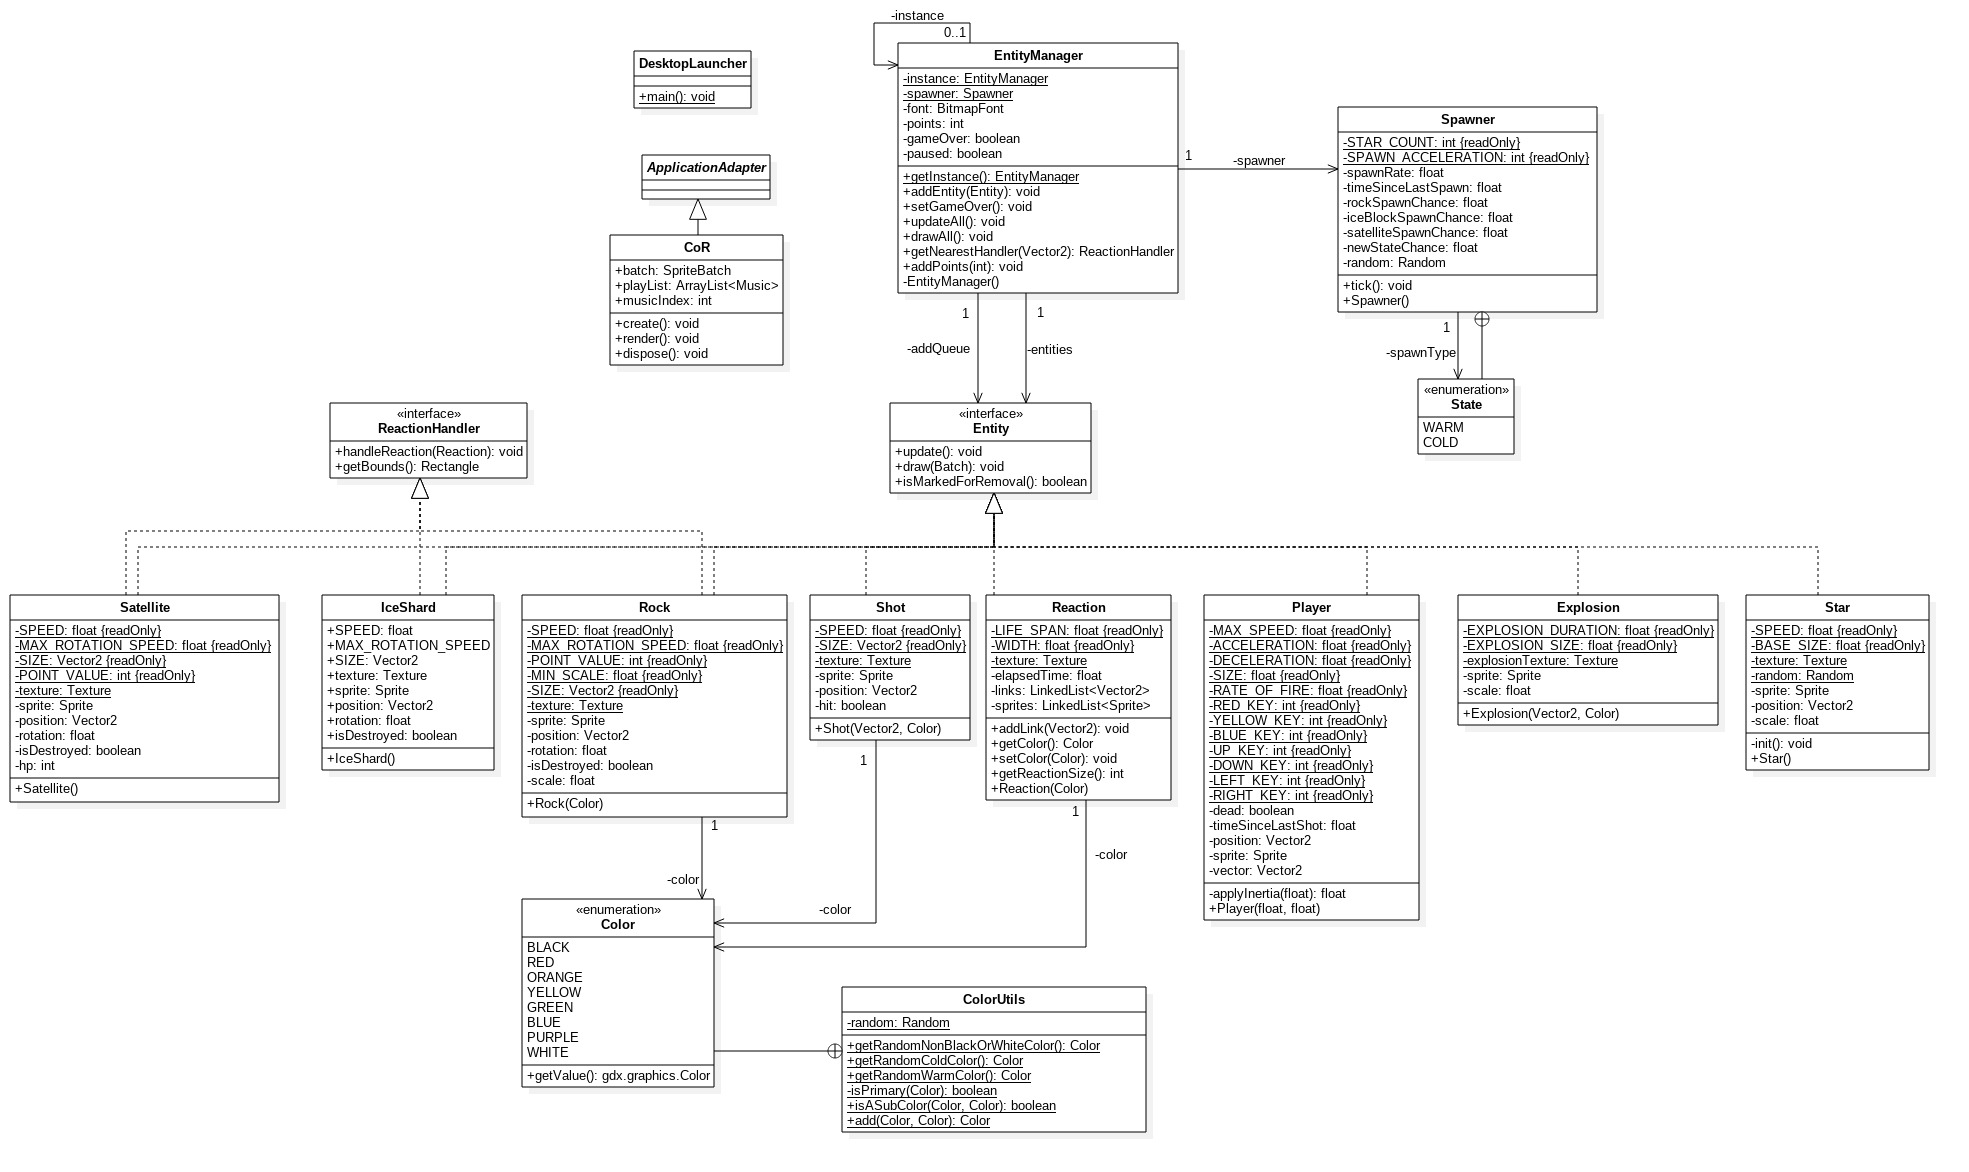
\includegraphics[width=\paperwidth,height=\paperheight,keepaspectratio,angle=90,origin=c]{uml_cor.jpg}

\clearpage

\section{Patrons de conception}
\subsection{Chaîne de responsabilité}
Les maillons de la chaîne de responsabilités sont les entités implémentant l'interface \texttt{ReactionHandler}. La requête qui est passée d'un maillon à l'autre est un objet de type \texttt{Reaction}.\\

\texttt{ReactionHandler} déclare les méthodes \texttt{handleReaction} (qui reçoit la requête) et \texttt{getBounds} (qui est nécessaire pour détecter une collision avec un élément de la chaîne). Lorsqu'un projectile entre en collision avec un \texttt{ReactionHandler}, il créé un objet \texttt{Reaction}, l'ajoute à l'\texttt{EntityManager}, puis l'envoie au \texttt{ReactionHandler} touché par le projectile.\\

La \texttt{Reaction} est passée de \texttt{ReactionHandler} en \texttt{ReactionHandler}. Elle peut être modifiée (longueur, couleur, aspect graphique), exploser/endommager un \texttt{ReactionHandler}, ou arrêtée (plus d'objet à l'écran ou couleur incompatible).

\subsection{Singleton}
Il a été décidé qu'\texttt{EntityManager} soit un singleton afin de permettre à n'importe quelle classe d'ajouter des entités à la boucle d'exécution du jeu. Elle permet également d'obtenir le \texttt{ReactionHandler} le plus proche d'une coordonnée spécifiée. La fin de vie d'une entité est signalée par cette dernière en renvoyant \textit{true} à l'appel de \texttt{isMarkedForRemoval}. C'est une façon simple de créer des entités, les faire vivre et mourir, sans avoir à gérer de multiples boucles d'exécutions interdépendantes (comme c'était le cas lors d'une première implémentation).

\subsection{Classe utilitaire}
\texttt{ColorUtils} est une classe utilitaire permettant de manipuler des objets du type énuméré \texttt{Color}. Comme ces manipulations sont sans états, et que toutes les valeurs reçues et renvoyées sont des constantes, nous avons décidé de rendre le constructeur privé et de ne pas forcer le paradigme objet sur cette classe.\\

Chaque élément de ce type prend une valeur de type \texttt{com.badlogic.gdx.graphics.Color} (\texttt{Color} définit par libgdx). Cette abstraction permet de définir des méthodes sur ces couleurs indépendamment de la couleur réelle affichée à l'écran. Par exemple \textbf{BLUE} et \textbf{RED} font \textbf{PURPLE}, mais les couleurs affichées sont \textbf{CYAN}, \textbf{RED} et \textbf{VIOLET}. Grâce à cette abstraction, ce mélange de couleur reste vrai même si on change la valeur de \textbf{BLUE} de \textbf{CYAN} à \textbf{SKY}.\\

\texttt{ColorUtils} possède donc des méthodes statiques pour mélanger deux couleurs, renvoyer une couleur aléatoire, ou savoir si une couleur est contenue dans une autre par mélange (cette dernière méthode n'est pas utilisée dans la version finale du jeu).

\clearpage

\section{Conclusion}
Bien que l'implémentation d'une chaîne de responsabilité dans le jeu était l'objectif principal du projet, un autre patron de conception (singleton) s'est naturellement glissés dans le code, contribuant à la clarté de la structure du programme. Cette dernière est restée simple car le jeu lui-même est minimaliste et quatre autres projets requéraient également du temps de travail.

\end{document}
